\uuid{3IbW}
\exo7id{5818}
\titre{exo7 5818}
\auteur{rouget}
\organisation{exo7}
\datecreate{2010-10-16}
\isIndication{false}
\isCorrection{true}
\chapitre{Conique}
\sousChapitre{Parabole}
\module{Géométrie}
\niveau{L2}
\difficulte{}

\contenu{
\texte{
Déterminer l'orthoptique d'une parabole, c'est-à-dire l'ensemble des points du plan par lesquels il passe deux tangentes à la parabole qui soient perpendiculaires.
}
\reponse{
\textbf{Solution géométrique.}

$$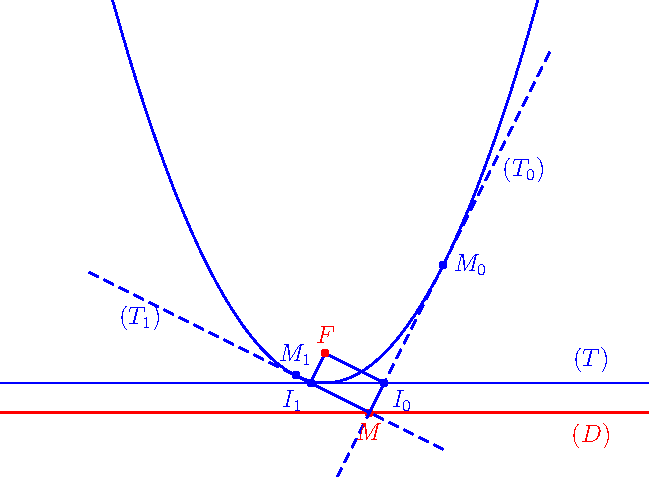
\includegraphics{../images/img005818-1}$$


Soit $M$ un point de l'othoptique. $M$ est sur les tangentes $(T_0)$ et $(T_1)$ à la parabole en deux points distincts $M_0$ et $M_1$ et clairement distinct du sommet $S$. Soient $I_0$ et $I_1$ les points d'intersection des droites $(T_0)$ et $(T_1)$ respectivement avec la tangente $(T)$ au sommet de la parabole. On sait (construction usuelle de la parabole par points et tangentes) que les droites $(T_0)$ et $(T_1)$ sont perpendiculaires aux droites $(FI_0)$ et $(FI_1)$ respectivement. Donc le quadrilatère $FI_0MI_1$ est un rectangle (3 angles droits connus). Par suite, le milieu de $[FM]$ qui est aussi le milieu de $[I_0I_1]$ est sur la tangente au sommet $(T)$ et $M$ est l'image d'un point de la tangente $(T)$ par l'homothétie de centre $F$ et de rapport $2$. Finalement, le point $M$ est sur la directrice de la parabole.

Réciproquement, soit $M$ un point de la directrice et $I$ le milieu de $[FM]$. On reconstruit le rectangle précédent en plaçant d'abord sur la tangente au sommet $(T)$ les points $I_0$ et $I_1$ tels que $I$ soit le milieu de $[I_0I_1]$ et tels que $I_0I_1 = MI$. Les droites $(MI_0)$ et $(MI_1)$ sont effectivement des tangentes à la parabole qui sont perpendiculaires l'une à l'autre.

\begin{center}
\shadowbox{
L'orthoptique d'une parabole est sa directrice.
}
\end{center}

\textbf{Solution analytique.} On choisit un repère orthonormé dans lequel la parabole a pour équation cartésienne $y^2=2px$. Une équation de la tangente $(T_0)$ à la parabole en un point $M_0=(x_0,y_0)=\left(\frac{y_0^2}{2p},y_0\right)$ est $-px_0+yy_0 = px_0$.

Deux tangentes $(T_0)$ et $(T_1)$ sont perpendiculaires si et seulement si $p^2 + y_0y_1 = 0$ (en particulier $y_0y_1\neq0$). Le point d'intersection des tangentes $(T_0)$ et (T1) en deux points distincts est la solution du système $\left\{
\begin{array}{l}
-px+yy_0=px_0\\
-px+yy_1=px_1
\end{array}
\right.$ et a donc pour coordonnées  $\left(\frac{p(x_0y_1-y_0x_1)}{p(y_0-y_1)},\frac{p^2(x_0-x_1)}{p(y_0-y_1)}\right)=\left(-\frac{y_0y_1}{2p},\frac{y_0+y_1}{2}\right)=\left(-\frac{p}{2},\frac{1}{2}\left(y_0-\frac{p^2}{y_0}\right)\right)$.

En résumé, un point $M(x,y)$  est sur l'orthoptique si et seulement si il existe $y_0\neq0$ tel que  
$\left\{
\begin{array}{l}
x=-\frac{p}{2}\\
y=\frac{1}{2}\left(y_0-\frac{p^2}{y_0}\right)
\end{array}
\right.$ ce qui montre déjà qu'un point de l'orthoptique est sur la droite d'équation $x = -\frac{p}{2}$  c'est-à-dire sur la directrice de la parabole. Réciproquement, la fonction $y_0\mapsto\frac{1}{2}\left(y_0-\frac{p^2}{y_0}\right)$ est continue sur $]0,+\infty[$, tend vers $-\infty$ quand $y_0$ tend vers $0$ par valeurs supérieures et tend vers $+\infty$ quand $y_0$ tend vers $+\infty$. Donc   $\frac{1}{2}\left(y_0-\frac{p^2}{y_0}\right)$ décrit $\Rr$ quand $y_0$ décrit $]0,+\infty[$, ce qui montre que l'on obtient la totalité de la directrice.
}
}
